\subsection{Bacical Calibration}

\begin{figure}[htbp]
  \begin{tabular}{cc}
    \begin{minipage}{0.5\hsize}
      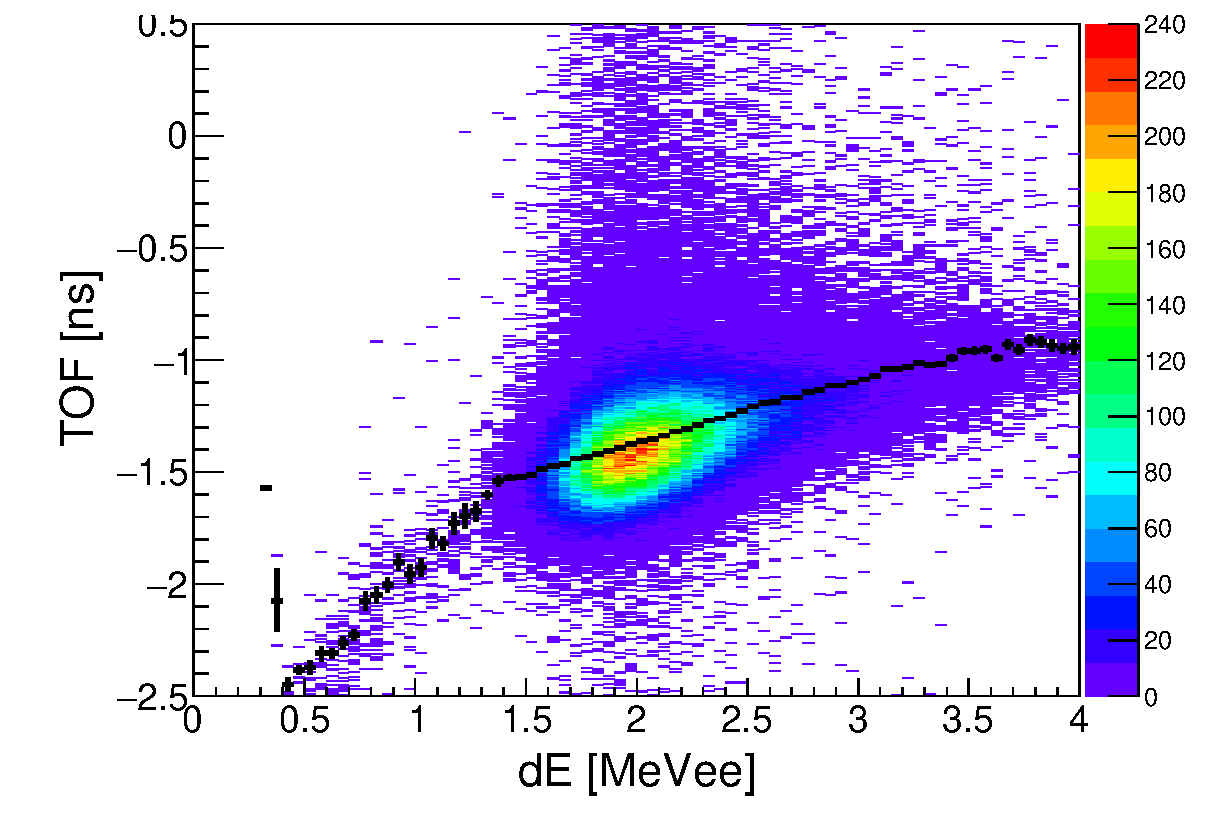
\includegraphics[width=5cm]{../pic/Dron/T0_slew_before.eps}
    \end{minipage}
    \begin{minipage}{0.5\hsize}
      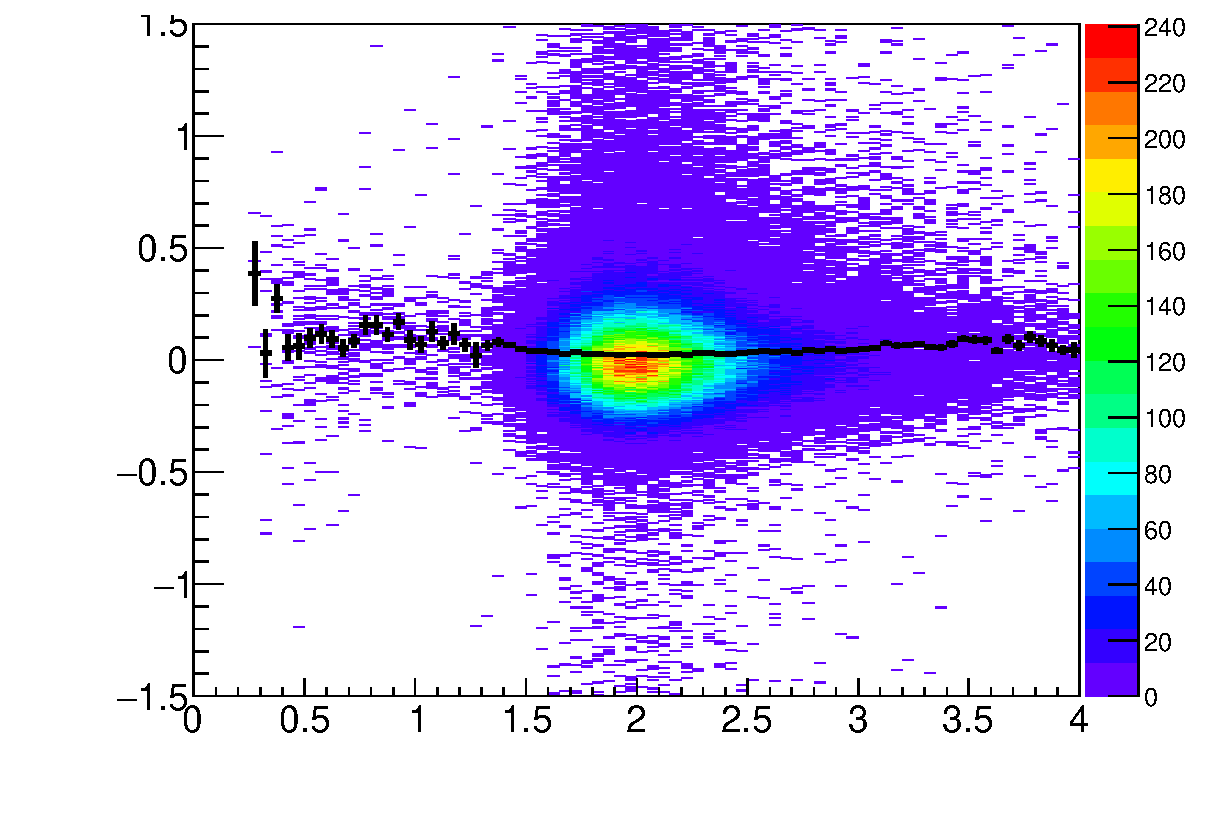
\includegraphics[width=5cm]{../pic/Dron/T0_slew_after.eps}
    \end{minipage}
  \end{tabular}

  \caption{
    These figures indicate about slewing effect correction.
    These figures show the energy deposit of the T0 as the horizontal axis and the calculated time shift of T0-NC by the γ-ray as the vertical axis.
    The left figure shows about before correction, and the right figure shows about after correction.
  }
  \label{fig:slew}
\end{figure}

This subsection describes basic detector corrections.
There are two types of data - ADC for the magnitude of the signal and TDC for the time, with the counter reading both ADC and TDC and the chamber reading only TDC.
The TDC signal 

Most counters are detectors for high-precision time information.
The TDC signal depends on the magnitude of the signal, as it is made from a digital signal where the raw signal is separated by a certain threshold value, as shown in left figure of Fig.\ref{fig:slew}.
A correction called slewing correction is used to compensate for this effect.
This correction uses the following as a function.
An example of the result at T0 is shown in Fig.\ref{fig:slew}.
The left figure shows the result before correction and the right figure shows the result after correction.

\begin{equation*}
  t_{corrected}=p_0+p_1 \frac{t}{\sqrt{dE}}+p_2 t
\end{equation*}

\begin{figure}[htbp]
  \centering
  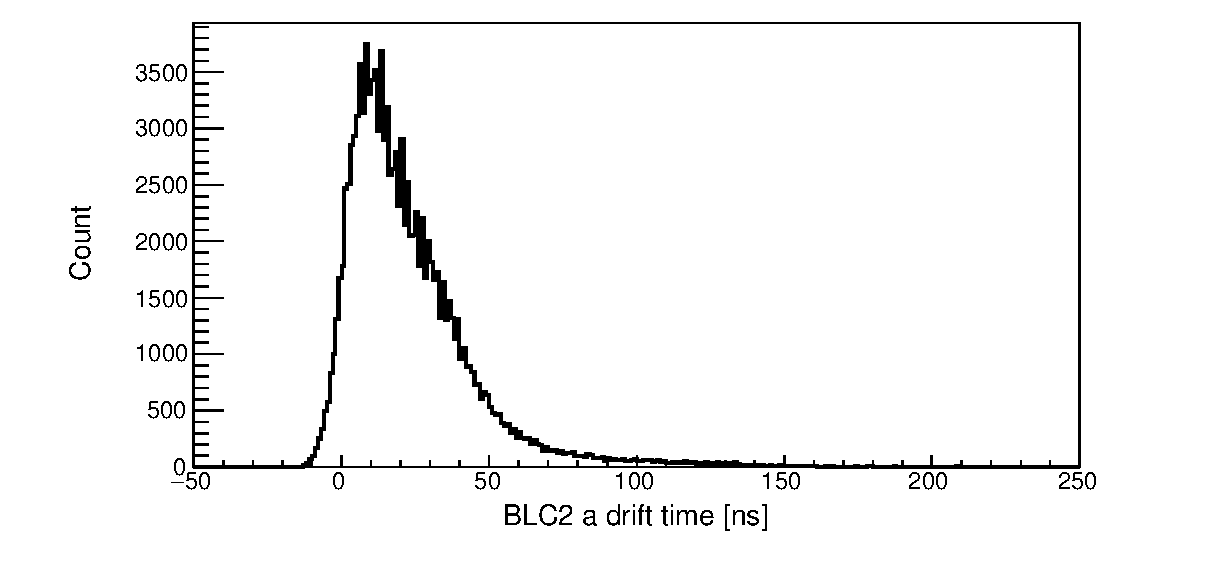
\includegraphics[width=10cm]{../pic/Dron/BLC2a_dt.eps}
  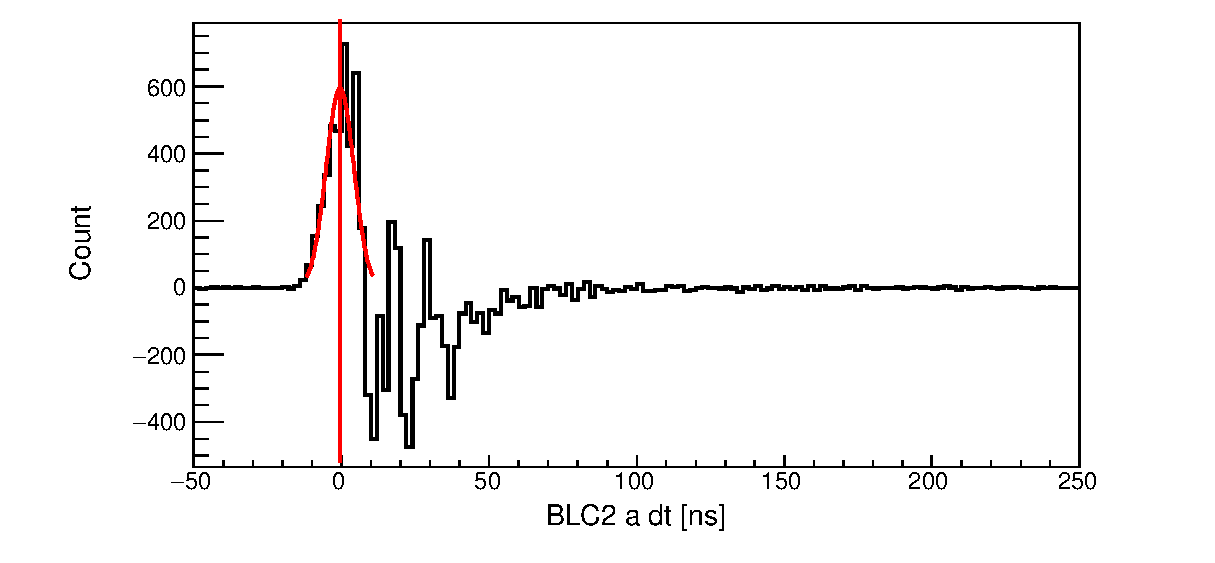
\includegraphics[width=10cm]{../pic/Dron/BLC2a_diff.eps}
  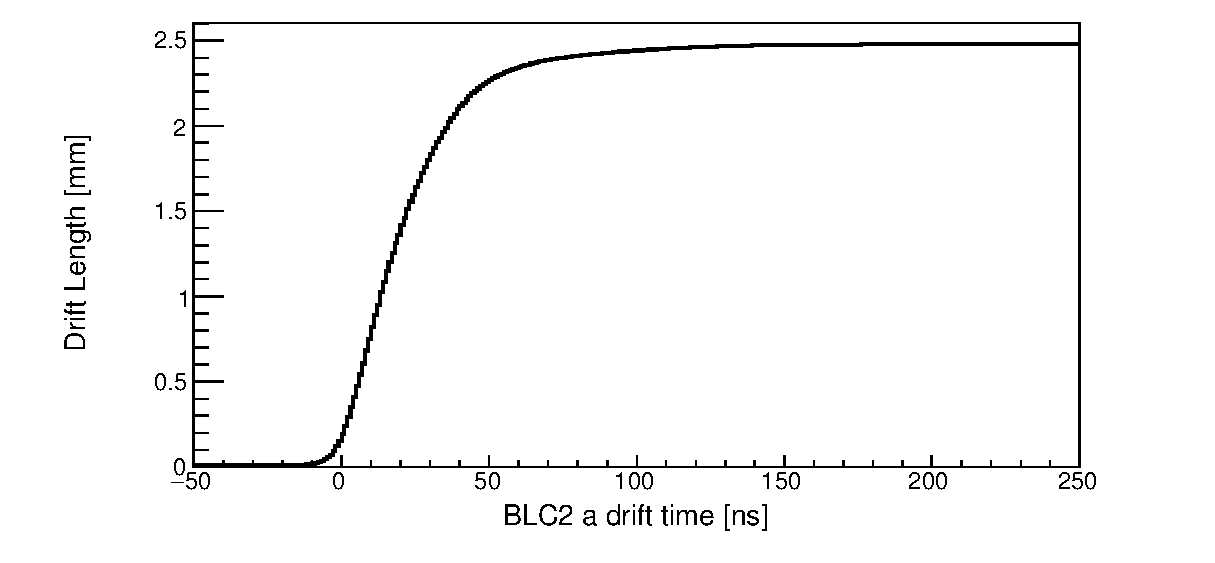
\includegraphics[width=10cm]{../pic/Dron/BLC2a_int.eps}
  \caption{
    These figures indicate the calibration of drift chambers.
    The above figure shows raw distribution.
    The middle figure shows the start timing decision which is indicated by red lines.
    The bottom figure shows the $x$-$t$ map.
  }
  \label{fig:BLDC_calib}
\end{figure}


The TDC signal of the chamber is converted to drift length.
Fig.\ref{fig:BLDC_calib} shows the conversion method.
By differentiating it, the rising edge of the signal is obtained, as shown in the middle figure.
The red line is used to determine the rising edge, the curve is the fitted Gaussian function and the vertical line is the rising point.
The conversion to drift length is done by integrating the TDC signal as shown in the down figurexs,
under the assumption that the charged particles are uniformly irradiated in the cells of the chamber.
This figure shows the $x\mbox{-}t$ map itself, which represents the correlation between the drift length and the drift time (TDC signal).
